\documentclass[12pt]{article}
\usepackage[utf8]{luainputenc}
\usepackage[danish]{babel}
\usepackage{listings}
\usepackage{amsfonts}
\usepackage{amsmath}
\usepackage{verbatim}
\usepackage{hyperref}
\usepackage[danish, colorinlistoftodos, textwidth=3cm]{todonotes}

\definecolor{secnum}{RGB}{102,102,102} 

\newcommand{\todolasse}[1]{\todo[color=green!40, inline]{#1}}
\newcommand{\todochristoffer}[1]{\todo[color=blue!40, inline]{#1}}

\title{sCT - working title}
\author{Christoffer Wadum Larsen\\
Lasse Ahlbech Madsen}
\begin{document}
\maketitle
\newpage
\tableofcontents
\newpage
\pagenumbering{arabic}

\listoftodos
\newpage

\section{Introduktion}

Til diagnosticering af patienter med visse former for sygdomme i hjerneregionen, fortages der ofte scanninger vha. Positron Emission Tomography (PET). 

PET scannere fungerer ved, at man injekterer et radioaktivt sporstof
ind i et legeme. Dette sporstof flyder ud i blodet og bliver bundet
der, hvor der benyttes mest energi, for eksempel en kræftcelle i
hjernen. Dette udsender stråling, som PET scanneren kan opfange.
Strålingsaktiviteten måles for at finde ud af, hvor i legemet der er
mest aktivitet.

PET har dog visse problemer. Man fanger kun strålingskoncentration,
så det er umuligt at se knogle, luft eller blødt væv. Dette giver
problemer, da forskelligt væv afbøjer photoner i forskellige grad,
og luft næsten ikke gør, forårsager det forringelser i kvaliteten
af scanningen, da man ikke er sikker på hvad photoner har bevæget
sig igenn, og dermed, hvor meget de er blevet afbøjet. Hvis man ikke
kender dette, kan man ikke med sikkerhed bestemme deres oprindelsessted.
Dette betragtes, som den væsentligste årsag til foringelse af
billederne.\cite{vigtighedAfAttenuation} At udbedre denne forringelse er
attenuationskorrigering.

For at udbedre denne forringelse har man kombineret Computed
Tomo\-graphy- (CT) og PET scannere. CT er et røngtenstrålingsscan,
der registrerer placering af knogle. Denne information kan man bruge
til at attenuationskorrigere og dermed få et mere korrekt resultat.
CT har dog andre problemer, da den ikke indeholder information om de
bløde vævstyper i hjernen. Derudover har røntgenstråling også
en væsentligt risiko for at forårsage yderlig skade. \cite{skadeligCT}

For at registrerer det bløde væv kan Magnetic Resonance(MR) benyttes.
MR magnetiserer et legeme svagt, når dette stoppes vil legemet hurtigt
gendanne sit oprindelige magnetfelt. Hastigheden med hvilken den gendannes
afhænger af vævet. MR scanneren varierer magnetiseringen og starter og
stopper det gentagne gange for at kortlægge legemet. Dette giver billeder
af hjernevæv i høj kvalitet.

Som med CT er MR også blevet sammensat med PET til en PET/MR scanner, men
den kan ikke bruges til attenuationkorrektion, da knogle og luft begge 
gendanner deres magnetfelt så hurtigt, at det er meget svært at måle.
Effekten er at knoglen kommer til at ligne luft på billederne. Dette
problem er forsøgt løst på flere måde.

På Rigshospitalet har man hidtil kombineret MR billeder med CT
billeder for at kunne lave attenuationskorrigerede billeder kaldet FullCT.
Dette medfører dog det tidligere nævnte problem med den skadende
effekt af røngtenstråling og man skal flytte patienten rundt mellem
flere scannere. Da scanningerne er foretaget på forskellige scannere
kan man ikke forvente at patienterne ligger ens. Dette problem skal
også løses. Derfor er man særdeles interesserede i, at foretage
attenuationskorrigering alene vha. MR.

Der er to hovedretninger til at udregne CT data ud fra MR data. De
anatomiske og de voxelbaserede. De anatomiske forsøger at kortlægge
hjernen og beskrive generelle træk, de matcher patient data op imod et
udregnet atlas, og forsøger at korrigere udfra det. Det giver nogle
problemer ved atypisk anatomi, men har vist sig at producere gode
resultater~\cite{atlas1, atlas2}.

Alternativt er der voxelbaserede metoder, som for hver voxel forsøger
at bestemme hvilken type væv den tilhører, men her er det selvfølgelig
virkelig et problem, at man ikke kan skelne mellem luft og knogle.

Ved at benytte meget korte sekvenser, kaldet UTE (Ultrashort Echo Times,)
er det muligt at registrere knogle på MR-scannere. Man måler fra to
forskellige vinkler og med to forskellige echo tider. Der hvor der er
sket en markant ændring i mellem de to billeder, kan da formodes at
være knogle. Implementation af dette på Siemens scannerne, som
Rigshospitalet benytter, har dog vist sig ikke at være på højde med
kombinationen af CT og MR billeder.

Målet med denne opgave er at implementere metoden beskrevet i
Johansson et al., som kan udregne et substitut-CT (sCT) ud fra fire
UTE sekvenser og et T2-vægtet MR billede for en vilkårlig patient. Dette
vil vi gøre ved at træne en Gaussian Mixture Regression model ud fra
disse serier samt et CT målt på samme patient.


\section{Teori}
\subsection{Kort introduktion til de forskellige type data og dannelse af disse.}

\todochristoffer{Læs}
\todolasse{Skriv om PET effekt på MR. Mere om forskel på UTE-sekvenserne}


Til metoden benyttes Magnetic resonance- (MR) og Computed
tomography-billedsekvenser (CT). CT er en røngtenscanning, som måler
evnen til at blokkere stråling, hvilket har en direkte relation til
elektrondensitet. Knoglen er meget tydelig i disse billeder. MR magnetiserer
kroppen ganske svagt, når dette stoppes vil kroppens magnetisering bruge
ganske kort tid på at gendannes, og der måles på denne for at kortlægge
struktur.

Vi benytter 5 MR-sekvenser: T1, som måles efter kroppen har gendannet en vis
mændge magnetisme, og derudover 4 Ultrashort echo time MR-sekvenser (UTE)
taget fra 2 forskellige vinkler og varierende ekko tider. Når man sænker echo
tiden betydeligt bliver det muligt at se knogle på MR billeder, men ikke med
en præcision, som kan matche CT.


\subsection{Registrering}

\todochristoffer{Mangler referencer i teori til registrering}

Billeder taget på PET/MR og PET/CT skannere kan som regelt ikke processeres
sammen grundet flere faktorer. Patienten ligger sjældent præcis på samme
måde, billederne bliver taget i forskellige opløsninger og patienten kan have
implantater der forvrænger billederne og de ligger også i forskellige image
spaces. For at klargøre billederne skal de derfor co-registreres.

Ved co-registrering forsøger man at få alle billederne til at ligge i samme
rum. I forhold til MRI billederne er co-registrering ofte trivielt. At
co-registrere et MRI og CT billede er derimod vanskeligere. Derfor har vi valgt
to forskellige metoder.

\todo{Mangler der noget her?}

I samme omgang som vi co-registrere billederne er vi interesserede også
at finde en maske. Masken skal bruges til at begrænse udregningen af sCT
billedet så vi ikke bruger lang tid på at lede efter knogle i luften rundt om
patienten.

\subsection{Attenuation correction}
Ved PET billeder måles photoner fra materiale man har sprøjtet ind i blodet. Ved
at se på hvor photonerne kommer fra kan man se hvor meget blod der flyder til
forskellige steder. Det er særligt brugbart til at identificere kræftknuder i
hjernen da kræftknuderne har et højere energiforbrug, og dermed får tilført
mere blod kan man se hvor de er henne.

Normalt bruges et CT billede for at korrigere for afbøjninger, men det  

\todochristoffer{Mangler at beskrive AC}

\subsection{Artifakter i hjerner}

\todo{Mangler at beskrive artifakter}

\subsection{Statistikgøjl}

\todochristoffer{Mangler at beskrive statistikken}

\todo{Overvej ordenen på næste 3 sections}

\subsection{Arbejdsgangen}

\todochristoffer{Arbejdsgangen er ikke beskrevet}

På Rigshospitalet er fremgangsmåden med MR
hjerneskanninger, at man også laver et CT scan. T1 billedet fra MR scanneren
og CT co-registreres herefter og sammenlægges til et attenuationskorrigeret
uMap kaldet FullCT. Derudover benyttes et Dixon uMap til at sætte dimensioner
på det nye uMap. Dette rekonstrueres på hospitalets scanner.


\subsubsection{FullCT}

\todolasse{FullCT er ikke beskrevet. Snakker nærmere med Claes og justerer
også i ovenstående snit}

Det er noget funk

\subsubsection{Rekonstruktion}

\todolasse{Rekonstruktion er ikke beskrevet. Skal snakke med et par folk.
Hvordan det }


\section{Registrering}

Billeder taget på MR/PET- og PET/CT-skannere kan som regel ikke
processeres sammen grundet flere faktorer. Patienten ligger sjældent
præcis på samme måde, billederne bliver taget i forskellige
opløsninger, og de bliver optaget i forskellige billedrum. For at
klargøre billederne skal de derfor co-registreres.

Ved co-registrering forsøger man at få alle billederne til at ligge i
samme rum. I forhold til MR-billederne er co-registrering ofte trivielt.
At co-registrere et MR- og CT-billede er derimod vanskeligere. Derfor har
vi valgt to forskellige metoder.

I samme omgang, som vi co-registrerer billederne, er vi interesserede i
også at finde en maske. Masken skal bruges til at lette udregningen
af sCT-billedet, så vi ikke bruger lang tid på at lede efter knogle i
luften rundt om patienten. Masken skal også fjerne eventuel nakkestøtte og
hovedholdere på CT-billederne.

\subsection{Co-registrering af UTE- og T2-billeder}

Til co-registrering af UTE- og T2-billederne har vi valgt at bruge
Insight ToolKit (ITK)\footnote{\url{http://www.itk.org/}}. Herfra benytter vi en implementation af Mattes
Mutual Information algoritme samt lineær translation og interpolering. Vi har valgt denne implementation fordi det var foreslået i dokumentationen for ITK.

\subsection{Co-registrering af UTE- og CT-billeder}

Co-registrering af UTE- og CT-billeder er, modsat UTE/T2, en ikke-triviel
opgave. Vi har valgt en landmark baseret løsning fra MINC's toolkit\footnote{\url{http://www.bic.mni.mcgill.ca/ServicesSoftware/ServicesSoftwareMincToolK it}}.
Vi har ikke selv skrevet denne løsning, men bruger i stedet samme
løsning som Rigshospitalet.

\subsection{Generering af maske}

Til udregning af modellerne har maskerne en væsentlig betydning for korrektheden af klassifikationen. Vi har flere gange undervejs måtte ændre hvilke billeder, som vi bruger til at genskabe modellerne, og har ikke haft tid til at generere de tilhørende masker hver gang.

Hvis ikke maskerne kun dækker punkter hvor der findes data på alle 16 billeder, risikerer vi en misklassificering. 

Til generering af masken bruger vi først en implementering af Otsu
thresholding-algoritmen for at finde en binær repræsentation. For at
sikre, at vores maske ikke bliver for lille, udvider vi det binære billede
vha. en neighborhood-connected-algoritme med 2-3 pixel i x, y og z
retningerne. Til sidst inverteres billedet, hvilket efterlader os med en
binær maske.

De endelige masker vi brugte var alt for store i forhold til T2-sekvenserne, hvilket kan have haft en betydelig negativ effekt på kvaliteten af vores T2.

Da det tager forholdsvis lang tid at udregne modellerne og endnu længere tid at lave rekonstruktionerne, havde vi ikke tid til at prøve med nye masker.



\section{Metoden}
\subsection{Gaussian Mixture Model}

\subsubsection{At finde modellen}
Vi bruger en mixtur af gaussians til at beregne voxel værdier
for et sCT. For hver patient har vi 5 MR-billeder og 1 CT billede.

For at øge præcisionen udregner vi for hvert MR-billede
to nye billeder. De nye billeder beregnes ved at se på en 3x3x3
kube omkring hvert voxel og finder henholdsvis middelværdi og varians.

Herefter har vi 15 MR-billeder og 1 CT-billede som vi vil klassificere
med en mixtur af gaussians. Fra Johannson et al. ved vi at vi kan få
gode resultater med 20 gaussiske fordelinger. 

For at finde parametrene til hver gaussiske fordeling bruger vi
Expectation-Maximization (EM) algoritmen på en sammensætning af patienter
vi vil træne på. Vi starter EM algoritmen med resultatet af k-means på
dataen, hvor k er sat til 20. Dette betyder at vi ikke behøver køre
EM-algoritmen flere gang og øger sandsynligheden for et godt resultat, da
dataen allerede er klassificeret.


\todochristoffer{Matematiske ekslempler}
\todolasse{Gennemlæs}


\subsubsection{Beregning af sCT}

Vi generere sCT værdierne ved at udregne den forventede værdi af CT baseret på de 15 MR billeder. 

Som beskrevet i Johanson et al., så udregnes den forventede værdi af CT ved

\begin{equation}
(X_1 | X_2 = x_2) = \frac{\Sigma^{N}_{i=1} \bar{\mu}_{1,i} a_i h_i(x_2)}{\Sigma^{N}_{i=1} a_i h_i(x_2)}
\end{equation}

Hvor $X_1$ er CT værdien, $X_2 = (X_2 \dots X_k)$ er MR værdierne, $a_i$ er blandingsforhold og $N$ er antallet af MR billeder samt

\begin{equation}
 \bar{\mu}_{1,i} = \mu_{1,i} + \Sigma_{1 2, i} \Sigma^{-1}_{22, i}(x_2 - \mu_{2,i})
\end{equation}
og
\begin{equation}
h_i(x_2)= \frac{1}{( 2 \pi )^{k/2}|\Sigma_{22,i}|^{1/2}}\exp^{-\frac{1}{2}(x_2 - \mu_{2,i})^T \Sigma^{-1}_{22, i}(x_2 - \mu_{2,i})}
\end{equation}

$\mu_{1,i}$, $\mu_{2,i}$, $\Sigma_{1 1, i}$, $\Sigma_{1 2, i}$, $\Sigma_{2 1, i}$, $\Sigma_{2 2, i}$ er værdierne $\mu_i$ og $\Sigma_i$ estimeret med EM algoritmen og segmenteret som

\begin{equation}
\mu_i = \left(\begin{array}{c}
\mu_{i,1} \\ 1 \times 1 \\
\mu_{i,1} \\ 1 \times (k - 1)  
\end{array}\right)
\end{equation} 
\begin{equation}
\Sigma_i = \left(\begin{array}{c c}
\Sigma_{11,i} & \Sigma_{12,i} \\ 1 \times 1  & 1 \times (k-1)\\
\Sigma_{21,i} & \Sigma_{22,i} \\ (k-1) \times 1  & (k-1) \times (k-1)\\  
\end{array}\right)
\end{equation}

\todolasse{Læs}

\subsection{Hvordan han vi valgt at implementere den}

\todochristoffer{Læs}

Til metoden benytter vi for hvert træningssæt et CT, en T2 vægtet MR-sekvens
og 4 MR UTE-sekvenser. Vi benytter Insight Toolkit (ITK) til at udregne et
billede med middelværdi og et med varians for hvert MR billede.

Disse henter vi ind i matlab, hvor vi benytter fitgmdist til at lave en
gaussisk mixture fordelingsmodel. Med denne kan vi udregne et sCT udfra den
samme slags MR-sekvenser vi brugte til at lave modellen, samt deres
mean- og variansbilleder.


\section{Praktisk}

\subsection{Beregning af modellen}

Vi har valgt at implementerer metoden i Matlab da det giver os mulighed for hurtig prototyping. Derudover indeholder Matlab også en standard implementering af både k-means og EM algoritmerne.

For at beregne modellen skal vi først indlæse MR og CT billederne samt tilhørende maske for hver patient. Til det formål har vi brugt nifti_load \todo{link til toolbox}.

Herefter løber vi billederne igennem og udtager de værdier der ligger inden for masken. Alle værdier lægges i én stor 16-dimensionel liste.

For at udregne k-means bruger vi den indbyggede k-means algoritme, samt en sammensat liste med de patienter vi ønsker til grund for modellen.

Output fra k-means algoritmen gives til EM algoritmen, samt samme liste med patienter. Output herfra er vores endelige model parametre.

\todo{inkludér kode snippets}

\subsection{Beregning af sCT}

\todochristoffer{Analysen af implementeringen er ikke beskrevet}


\section{Forsøg}

\subsection{Hvordan vil vi vurdere resultatet}

For at validere testresultaterne vil vi benytte os af joint histograms. For hvert sCT vi generer har vi det korrekte CT. Ved at plotte sCT værdier som x koordinaten og CT værdier som y koordinaten får vi en visuel repræsentation af ligheden mellem billederne. Hvis resultatet er identisk vil der optræde en enkelt lige linje fra (0,0) til (max,max). Jo mere forskellige de er jo længere fra den lige linje ligger punkterne.

Fordelen ved denne metode er at vi nemt kan aflæse hvilke værdier vi har de største problemer med. Hvis vi har meget stor afvigelse i knoglerne vil vi få en stor klump omkring nul, mens der kan være store ligheder i det bløde væv der så giver en pæn linje omkring minus 500.

Derudover er det samme valideringsmetode der bruges af Johannson et al., og vi vil derfor kunne sammenligne vores værdier med deres.

For at finde ud af om vores sCT er godt nok til attenuationskorrektion af PET billeder vil vi generere PET billeder med vores sCT og det rigtige CT. Vi kan herefter konstruere et nyt billede, der er baseret på den procentvise forskel imellem PET/CT og PET/sCT. 

Ud fra procentsforskelsbilledet kan vi se hvilke regioner der er forskellige fra PET/CT billedet, og giver samtidigt et godt overblik over hvor godt vores PET/sCT billede er blevet.

Begge disse valideringsmetoder er objektive men skal valueres manuelt. Vi har ikke en metode til at give et enkelt tal for hvor godt vores PET/sCT billede er blevet. Vi forventer også at kvaliteten af sCT billedet, og dermed også PET/sCT billedet vil variere meget.

\todolasse{Læs}

\subsection{Planlagte forsøg}

\subsubsection{Leave-one-out cross validation (LOOCV)}
\paragraph{Fremgangsmåde}
Ved Leave-One-Out-Cross-Validation (LOOCV) tager vi et mindre dataset på fem patienter.

Ud af de fem patienter tager vi fire patienter og bruger dem til at træne algoritmen. Træningsparametrene her fra benytter vi til beregning af sCT billedet for den femte patient.

Samme procedure gentages fem gange så vi i alt har fem sCT billeder til fem forskellige patienter.

Vi har valgt dette test scenarie for at kunne sammenligne vores resultater med Johansson et al, da de benytter samme test.

\todolasse{Læs}

\paragraph{Forventning}
Vi forventer, at vores resultater bliver nogenlunde ens med Johansson et al.

\paragraph{Resultat}
\todo{Udfør LOOCV-forsøget}

\begin{figure}
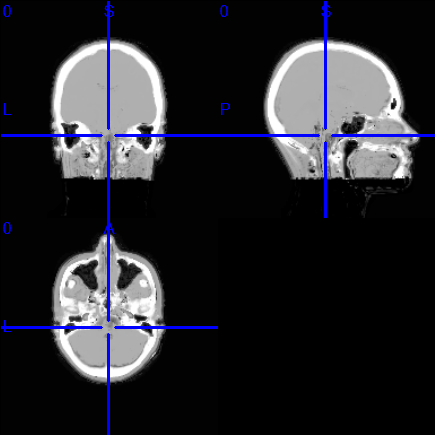
\includegraphics[width=\linewidth]{sct0.png}
\caption{sct0.png}
\end{figure}

\begin{figure}
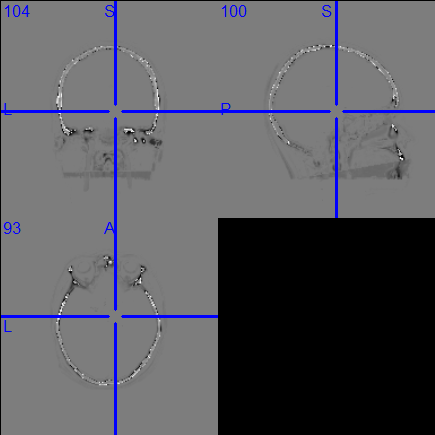
\includegraphics[width=\linewidth]{pdsct0.png}
\caption{Procent difference med værdier +- 100 sat til +- 100.}
\end{figure}

\begin{figure}
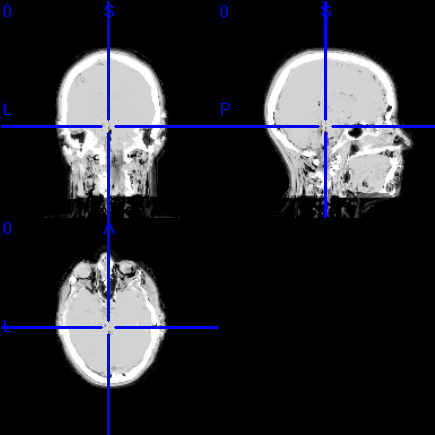
\includegraphics[width=\linewidth]{sct1.png}
\caption{sct1.png}
\end{figure}

\begin{figure}
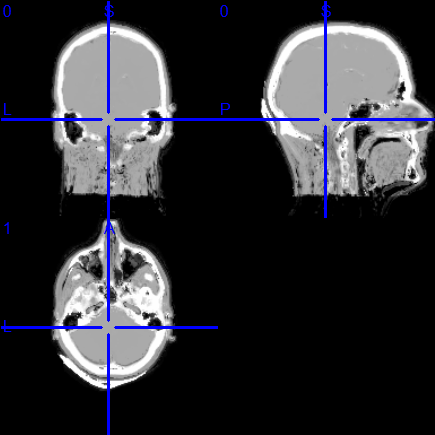
\includegraphics[width=\linewidth]{sct5.png}
\caption{sct5.png}
\end{figure}

\subsubsection{Udregn sCT til hjerner med artifakter trænet på hjerner uden artifakter}
\paragraph{Fremgangsmåde}
Træn på n hjerner test på m.

\paragraph{Forventning}

\paragraph{Resultat}

\subsubsection{Udregn sCT til hjerner trænet på hjerner med artifakter}
\paragraph{Fremgangsmåde}
Iterativt træn på et antal hjerner og introducer hjerner med artifakter.
Sammenlign kvaliteten af sCT afhængigt af andelen af hjerner, som har
artifakter.

\paragraph{Forventning}
At sCT's kvalitet forværes for hver introduceret hjerne med artifakt.

\paragraph{Resultat}


\subsubsection{Over tid}
\paragraph{Fremgangsmåde}
Træn på gamle hjerner, test på ny hjerner. Og omvendt.

\paragraph{Forventning}
Forventningen er sCT af samme kvalitet, som dem ved LOOCV-forsøget.

\paragraph{Resultat}

\subsubsection{Test på en masse}
\paragraph{Fremgangsmåde}
Iterativt træn på n+1 hjerner

\paragraph{Forventning}
Forventning er at efter 7-8 hjerner giver det ikke rigtig nogen
kvalitetsforskel.

\paragraph{Resultat}

\section{Vurdering}
\subsection{Kvalitet}

\todolasse{Kvaliteten af vores implementering er ikke beskrevet}

\subsection{Problemer fx. Artifakter}

\todolasse{Har ikke skrevet om problemer i forhold til sCT}

\subsection{Over tid}

\todolasse{Har ikke beskrevet korrektheden over tid}

\section{Konklusion}

Vores implementering af metoden til udregning af sCT beskrevet i Johansson
et. al. lever ikke op til deres resultater. Vi får større udslag i forhold
til CT-billederne end de gør, og på PET billederne måler vi for store
forskelle i forhold til dem, som er rekonstrueret med FullCT.  Metoden vil
måske kunne bruges til hukommelsespatienter, hvor man hovedsageligt
registrerer regionale forskelle, men ikke til patienter med hjernekræft,
hvor der skal lokaliseres aktivitetsknuder i hjernen.

Over tid ser der ud til at ske en værdiforskydning i PET billederne, som
giver lavere værdi i sCT, jo nyere patienter modellen er trænet på. Det
betyder lavere attenuering og dermed højere værdier i de rekonstruerede
PET billeder. Derfor må det anses som nødvendigt at træne nye modeller
løbende.

Vi har undervejs i projektet lavet nogle fejl, og vi har redegjort for
muligheder for at forbedre implementeringen, så bedre resultater burde
være mulige.




\end{document}
